\documentclass[a4paper, 12pt]{article}

\def\languages{french, english}

%%%%%%%%%%%%%%%%%%% Libraries

%%%%%%%%%% Packages

%%%%% Coding tools

\usepackage{comment}
\usepackage{xstring}

%%%%% Encoding

\usepackage[utf8]{inputenc}
\usepackage[T1]{fontenc}
\usepackage{eurosym}

%%%%% Languages

\ifx\languages\undefined
	\usepackage[english]{babel}
\else
	\usepackage[\languages]{babel}
\fi

\def\languagefile{./include/languages/\languagename.tex}
\InputIfFileExists{\languagefile}{}

%%%%% Style

\usepackage{geometry}
\usepackage{fancyhdr}
\usepackage[bottom]{footmisc}

\edef\restoreparindent{\parindent=\the\parindent\relax}
\usepackage[parfill]{parskip}

\usepackage{enumitem}
\usepackage{csquotes}
\usepackage{color}

%%%%% Others

\usepackage[framemethod=TikZ]{mdframed}
\usepackage[pdfusetitle]{hyperref}

%%%%%%%%%% Features

%%%%% Settings

\geometry{paper=a4paper,top=3.5cm,bottom=2.5cm,right=2.5cm,left=2.5cm}

\pagestyle{fancy}
\fancyhead[L]{}
\fancyhead[R]{\leftmark}
\fancyfoot[C]{\thepage}
\renewcommand{\headrulewidth}{0pt}

%\restoreparindent

%%%%% Commands

\newcommand{\romantableofcontents}{
	\newpage
	\pagenumbering{roman}
	\tableofcontents
	\newpage
	\pagenumbering{arabic}
}

%%%%%%%%%% Packages

\usepackage{float}
\usepackage[skip=1em]{caption}
\usepackage{subcaption}

\usepackage{array}
\usepackage{multirow}
\usepackage{multicol}

%%%%%%%%%% Features

%%%%% Settings

\renewcommand{\arraystretch}{1.2}

%%%%% Commands

\newcommand\noskipcaption[1]{\caption{#1}\vspace{-1em}}
\newcommand\noskipcaptionstar[1]{\caption*{#1}\vspace{-1em}}

%%%%%%%%%% Packages

\usepackage{amsmath}
\usepackage{amssymb}
\usepackage{bm}
\usepackage{esint}
\usepackage[makeroom]{cancel}

%%%%%%%%%% Features

%%%%% Macros

\newcommand{\rbk}[1]{\left(#1\right)}
\newcommand{\cbk}[1]{\left\{#1\right\}}
\newcommand{\sbk}[1]{\left[#1\right]}
\newcommand{\abs}[1]{\left|#1\right|}
\newcommand{\norm}[1]{\left\|#1\right\|}

\newcommand{\fact}[1]{#1!}
\newcommand{\e}[1]{\mathbf{e}_{#1}}
\newcommand{\deriv}{\mathrm{d}}
\DeclareMathOperator{\tr}{tr}

\def\Rl{\mathbb{R}}
\def\Cx{\mathbb{C}}
\def\Na{\mathbb{N}}
\def\Zi{\mathbb{Z}}

%%%%%%%%%% Packages

\usepackage{siunitx}

%%%%%%%%%% Features

%%%%% Settings

\ifx\decimalsign\undefined
\else
    \sisetup{output-decimal-marker = \decimalsign}
\fi


%%%%%%%%%%%%%%%%%%% Titlepage

\title{\vspace{-2cm}\textsc{ELEN0062} - Introduction to machine learning\\Project 2 - Bias and variance analysis}
\author{
François \textsc{Rozet} (s161024)\\
Adrien \textsc{Schoffeniels} (s162843)\\
}
\date{\today}

%%%%%%%%%%%%%%%%%%%

\newcommand{\X}{\mathcal{X}}
\newcommand{\Y}{\mathcal{Y}}
\newcommand{\Z}{\mathcal{Z}}
\DeclareMathOperator{\argmax}{argmax}
\DeclareMathOperator{\argmin}{argmin}

\DeclareMathOperator{\arctantwo}{arctan2}

%%%%%%%%%%%%%%%%%%%

\begin{document}
	\maketitle
	
	\section{Bayes model and residual error in classification}
	\begin{enumerate}[label = (\alph*)]
	    \item Using the conditional probability definition, the Bayes model becomes
    	\begin{align*}
    	    h_b(x_0, x_1) & = \argmax_y P_{y}(y \mid x_0, x_1) \\
    	    & = \argmax_y \frac{P_y(y)}{p_{x_0,x_1}(x_0, x_1)} p_{x_0,x_1}(x_0, x_1 \mid y) \\
    	    & = \argmax_y P_{y}(y) \, p_{x_0,x_1}(x_0, x_1 \mid y)
    	\end{align*}
    	where $p$ represents a density probability and $P$ a probability.
    	But we know that $$x_0 = r \cos \alpha \text{ and } x_1 = r \sin \alpha$$ with $r \in \Rl$ and $\alpha \in [0, 2\pi]$. Therefore, $$ p_{x_0, x_1}(x_0, x_1 \mid y) = \sum_{i} \frac{p_{r, \alpha}\rbk{r_i, \alpha_i \mid y}}{\abs{\det J\rbk{r_i, \alpha_i}}} $$ where $J$ is the Jacobian matrix of the transformation $(r, \alpha) \mapsto (x_0, x_1)$, i.e
    	$$
    	J(r, \alpha) =
    	\begin{pmatrix}
    	    \cos \alpha & -r \sin \alpha \\
    	    \sin \alpha & r \cos \alpha \\
    	\end{pmatrix}
    	$$ and where all pairs $(r_i, \alpha_i)$ are solutions of $$x_0 = r_i \cos \alpha_i \text{ and } x_1 = r_i \sin \alpha_i \, .$$
    	There exist two such pairs : $$\rbk{\sqrt{{x_0}^2 + {x_1}^2}, \arctantwo(x_1, x_0)} \text{ and } \rbk{-\sqrt{{x_0}^2 + {x_1}^2}, \arctantwo(-x_1, -x_0)} \, .$$
    	Also,
    	$$
    	\det J(r, \alpha) =
    	\begin{vmatrix}
    	    \cos \alpha & -r \sin \alpha \\
    	    \sin \alpha & r \cos \alpha \\
    	\end{vmatrix}
    	= r \, .
    	$$
    	Hence, $$ p_{x_0, x_1}(x_0, x_1 \mid y) = \frac{1}{\bar{r}} \sbk{p_{r, \alpha}\rbk{\bar{r}, \bar{\alpha}_+ \mid y} + p_{r, \alpha}\rbk{-\bar{r}, \bar{\alpha}_- \mid y}} $$
    	where $\bar{r} = \sqrt{{x_0}^2 + {x_1}^2}$ and $\bar{\alpha}_\pm =  \arctantwo(\pm x_1, \pm x_0)$.

    	But, from the statement, it is known that
    	\begin{align*}
    	    y & \sim \mathcal{U}\cbk{-1,+1} & r & \sim \mathcal{N}(R^y, \sigma^2) & \alpha & \sim \mathcal{U}(0, 2 \pi)
    	\end{align*}
    	which yield
    	\begin{align*}
    	    P_y(y) & = \frac{1}{2} \\
    	    p_\alpha(\alpha \mid y) & = p_\alpha(\alpha) = \frac{1}{2\pi} \\
    	    p_r(r \mid y) & = \frac{1}{\sqrt{2 \pi \sigma^2}} \exp\rbk{-\frac{(r - R^y)^2}{2 \sigma ^2}} \\
    	    p_{r, \alpha}(r, \alpha \mid y) & =  p_{r}(r \mid y) \, p_{\alpha}(\alpha \mid y) \, .
    	\end{align*}
    	Then, injecting all the above in the previous expression of $h_b(x_0, x_1)$, one obtains
    	\begin{align*}
    	    h_b(x_0, x_1) & = \argmax_y \frac{1}{4 \pi} \frac{1}{\bar{r}} \frac{1}{\sqrt{2 \pi \sigma^2}} \sbk{\exp\rbk{-\frac{(\bar{r} - R^y)^2}{2 \sigma ^2}} + \exp\rbk{-\frac{(\bar{r} + R^y)^2}{2 \sigma ^2}}} \\
    	    & = \argmax_y \exp\rbk{-\frac{(\bar{r} - R^y)^2}{2 \sigma ^2}} + \exp\rbk{-\frac{(\bar{r} + R^y)^2}{2 \sigma ^2}} \, .
    	\end{align*}
    	Therefore, $h_b(x_0, x_1) = 1$ if $\bar{r}$ is greater than $z$ such that
    	\begin{align*}
    	    \exp\rbk{-\frac{(z - R^+)^2}{2 \sigma ^2}} & + \exp\rbk{-\frac{(z + R^+)^2}{2 \sigma ^2}} \\
    	    & = \exp\rbk{-\frac{(z - R^-)^2}{2 \sigma ^2}} + \exp\rbk{-\frac{(z + R^-)^2}{2 \sigma ^2}} \, .
    	\end{align*}
    	Supposing $R^+ > R^- \gg 0$, one can show that $z \in \sbk{R^-, R^+}$. However, since $\sigma^2 = \num{0.1}$ , the exponentials of
    	$-\frac{(z + R^y)^2}{2 \sigma ^2}$ are negligible in front of the exponentials of $-\frac{(z - R^y)^2}{2 \sigma ^2}$ within the interval $\sbk{R^-, R^+}$.
    	
    	Thus, using this approximation,
    	\begin{alignat*}{2}
    	    && \exp\rbk{-\frac{(z - R^+)^2}{2 \sigma ^2}} & = \exp\rbk{-\frac{(z - R^-)^2}{2 \sigma ^2}} \\
    	    \Leftrightarrow \quad &&  -\frac{(z - R^+)^2}{2 \sigma ^2} & = -\frac{(z - R^-)^2}{2 \sigma ^2} \\
    	    \Leftrightarrow \quad &&  (z - R^+)^2 & = (z - R^-)^2 \\
    	    \Leftrightarrow \quad &&  z^2 - 2 z R^+ + {R^+}^2 & = z^2 - 2 z R^- + {R^-}^2 \\
    	    \Rightarrow \quad &&  z & = \frac{{R^+}^2 - {R^-}^2}{2 (R^+ - R^-)} = \frac{R^- + R^+}{2} \, .
    	\end{alignat*}
        Finally,
    	\begin{align}
    	    h_b(x_0, x_1) & = 
    	    \left\{
    	    \begin{aligned}
    	        & +1 && \text{if } \bar{r} \geq z = R^\pm \\
    	        & -1 && \text{else}
    	    \end{aligned}
    	    \right.
    	\end{align}
    	where $R^\pm = \frac{R^- + R^+}{2}$.

    	\item Using the fact that
    	$$E\cbk{1(x)} = P(x)$$
    	the residual error becomes
    	\begin{align*}
    	    E_{x_0, x_1, y}\cbk{1\rbk{y \neq h_b(x_0, x_1)}} & = P(y \neq h_b(x_0, x_1)) \\
    	    & = \sum_y P_y(y) \, P(y \neq h_b(x_0, x_1) \mid y) \\
    	    & = P_y(-1) \, P(\bar{r} >  R^\pm \mid -1) + P_y(1) \, P(\bar{r} \leq  R^\pm \mid 1)
    	\end{align*}
    	But $\bar{r} = \abs{r}$ and $P_y(-1) = P_y(1) = \frac{1}{2}$. Therefore,
    	\begin{align}
    	    E_{x_0, x_1, y} & \cbk{1\rbk{y \neq h_b(x_0, x_1)}} \nonumber \\
    	    & = \frac{1}{2} \sbk{1 - P(-R^\pm \leq r \leq  R^\pm \mid -1)} + \frac{1}{2} P(-R^\pm \leq r \leq  R^\pm \mid 1) \nonumber \\
    	    & = \frac{1}{2} + \frac{1}{2} \int_{-R^\pm}^{R^\pm} \sbk{ p_r(r \mid 1) - p_r(r \mid -1) } \deriv r \nonumber \\
    	    & = \frac{1}{2} + \frac{1}{2} \int_{-R^\pm}^{R^\pm} \frac{1}{\sqrt{2 \pi \sigma^2}} \sbk{ \exp\rbk{-\frac{\rbk{r - R^+}^2}{2 \sigma ^2}} - \exp\rbk{-\frac{\rbk{r - R^-}^2}{2 \sigma ^2}}} \deriv r
    	\end{align}
    	whose second term is a finite (Gaussian) integral computable numerically. Indeed, using Python's \texttt{scipy.integrate.quad} function,
    	\begin{align}
    	    E_{x_0, x_1, y} \cbk{1\rbk{y \neq h_b(x_0, x_1)}} & = \num{0.0569}
    	\end{align}
	\end{enumerate}
	
	\section{Bias and variance of the \emph{kNN} algorithm}\label{sec:bias_variance_knn}
	\begin{enumerate}[label = (\alph*)]
	    \item As seen in the theoretical lectures,
	    \begin{align*}
	       E_{LS} & \cbk{E_{y \mid \bm{x}}\cbk{(y - \hat{y}(\bm{x}))^2}} \\
	       & = E_{LS}\cbk{E_{y \mid \bm{x}}\cbk{(y - E_{y \mid \bm{x}}\cbk{y} + E_{y \mid \bm{x}}\cbk{y} - \hat{y}(\bm{x}))^2}} \\
	       & = E_{LS}\cbk{E_{y \mid \bm{x}}\cbk{(y - E_{y \mid \bm{x}}\cbk{y})^2}} + E_{LS}\cbk{E_{y \mid \bm{x}}\cbk{(E_{y \mid \bm{x}}\cbk{y} - \hat{y}(\bm{x}))^2}} \\
	       & + E_{LS}\cbk{E_{y \mid \bm{x}}\cbk{2(y-E_{y \mid \bm{x}}\cbk{y})(E_{y \mid \bm{x}}\cbk{y}- \hat{y}(\bm{x}))}} \\ 
	       & = E_{y \mid \bm{x}}\cbk{(y - E_{y \mid \bm{x}}\cbk{y})^2} + E_{LS}\cbk{(E_{y \mid \bm{x}}\cbk{y} - \hat{y}(\bm{x}))^2} + 0 \\
	       & = V_{y \mid \bm{x}} \cbk{y} + E_{LS}\cbk{(E_{y \mid \bm{x}}\cbk{y} - \hat{y}(\bm{x}))^2} \\
	       & = V_{y \mid \bm{x}} \cbk{y} + E_{LS}\cbk{(E_{y \mid \bm{x}}\cbk{y} - E_{LS} \cbk{\hat{y}(\bm{x})} + E_{LS} \cbk{\hat{y}(\bm{x})} - \hat{y}(\bm{x}))^2} \\
	       & = V_{y \mid \bm{x}} \cbk{y} + E_{LS}\cbk{(E_{y \mid \bm{x}}\cbk{y} - E_{LS} \cbk{\hat{y}(\bm{x})})^2} + E_{LS}\cbk{(E_{LS} \cbk{\hat{y}(\bm{x})} - \hat{y}(\bm{x}))^2} \\
	       & + E_{LS}\cbk{2 (E_{y \mid \bm{x}}\cbk{y} - E_{LS} \cbk{\hat{y}(\bm{x})})(E_{LS} \cbk{\hat{y}(\bm{x})} - \hat{y}(\bm{x}))} \\
	       & = V_{y \mid \bm{x}} \cbk{y} + \rbk{E_{y \mid \bm{x}}\cbk{y} - E_{LS} \cbk{\hat{y}(\bm{x})}}^2 + E_{LS}\cbk{(\hat{y}(\bm{x}) - E_{LS} \cbk{\hat{y}(\bm{x})})^2} + 0 \\
	       & = V_{y \mid \bm{x}} \cbk{y} + \rbk{E_{y \mid \bm{x}} \cbk{y} - E_{LS} \cbk{\hat{y}(\bm{x})}}^2 + V_{LS} \cbk{\hat{y}(\bm{x})}
	    \end{align*}
	    where, knowing $y = f(\bm{x}) + \epsilon$,
	    $$\hat{y}(\bm{x}) = \hat{y}(\bm{x}; LS, k) = \frac{1}{k} \sum_{l = 1}^{k} f(\bm{x}_{(l)}) + \epsilon_l \, .$$
	    Keeping in mind that the expectation of a constant\footnote{Evaluating the model at $\bm{x}$, all $\bm{x}_l$ are constant with respect to $LS$.} is itself and its variance is $0$,
	    \begin{align*}
	        V_{y \mid \bm{x}} \cbk{y} & = V_{y \mid \bm{x}} \cbk{f(\bm{x})} + V_{y \mid \bm{x}} \cbk{\epsilon} = 0 + \sigma^2 \\
	        V_{LS} \cbk{\hat{y}(\bm{x})} & = \frac{1}{k^2} \sum_{l = 1}^{k} \rbk{ V_{LS} \cbk{f(\bm{x}_{(l)})} + V_{LS} \cbk{\epsilon_l}} = \frac{1}{k^2} \sum_{l = 1}^{k} \rbk{0 + \sigma^2} \\
	        E_{y \mid \bm{x}} \cbk{y} & = E_{y \mid \bm{x}} \cbk{f(\bm{x})} + E_{y \mid \bm{x}} \cbk{\epsilon} = f(\bm{x}) + 0 \\
	        E_{LS} \cbk{\hat{y}(\bm{x})} & = \frac{1}{k} \sum_{l = 1}^{k} \rbk{E_{LS} \cbk{f(\bm{x}_{(l)})} + E_{LS} \cbk{\epsilon_l}} = \frac{1}{k} \sum_{l = 1}^{k} \rbk{f(\bm{x}_{(l)}) + 0}
	    \end{align*}
	    which trivially yields
	    \begin{align}
	       E_{LS}\cbk{E_{y \mid \bm{x}}\cbk{(y - \hat{y}(\bm{x}))^2}} & = \sigma^2 + \sbk{f(\bm{x}) - \frac{1}{k} \sum_{l = 1}^{k} f(\bm{x}_{(l)})}^2 + \frac{\sigma^2}{k} \label{eq:bias_variance_decomposition_knn}
	    \end{align}
	    supposing $k \leq N$.
	    \item The bias-variance decomposition \eqref{eq:bias_variance_decomposition_knn} is composed of three parts :
	    \begin{enumerate}[label = \arabic*.]
	        \item $\sigma^2$, the \emph{noise} of the class $y$ knowing $\bm{x}$. This term is independent of the classification model and therefore of $k$. Indeed, $\sigma^2$ doesn't vary with $k$.

	        \item $f(\bm{x}) - \frac{1}{k} \sum_{l = 1}^{k} f(\bm{x}_{(l)})$, the \emph{bias} (squared in the decomposition) of the model. The right term is the mean of $f$ over the $k$ nearest neighbours of $\bm{x}$.
	        
	        When $k$ increases, this mean tends towards the mean of $f$ over all input values and reaches it for $k = N$. If in addition $N \rightarrow \infty$, the bias becomes the difference between $f(\bm{x})$ and its mean $E_{\bm{x}}\cbk{f(\bm{x})}$.
	        
	        \item $\frac{\sigma^2}{k}$, the \emph{variance} of the model. This term corresponds to the variance of $k$ independent drawing of $\epsilon$ which obviously decreases when $k$ increases.
	    \end{enumerate}
	\end{enumerate}
	
    \section{Bias and variance estimation}
    \begin{enumerate}[label=(\alph*)]
        \item Let $LS = \cbk{(\bm{x}_i, y_i) \mid i = 1, \ldots, N}$ (with $\bm{x}_i \in \Rl^p$ and $y_i \in \Rl$) denote a given learning sample (of size $N$) and $\hat{y}(\bm{x})$ denote the function learned from $LS$ by the given supervised algorithm. As seen before, it is known that
        \begin{align*}
            \text{noise}(\bm{x}) & = V_{y \mid \bm{x}} \cbk{y} = E_{y \mid \bm{x}} \cbk{\rbk{y - E_{y \mid \bm{x}}\cbk{y}}^2} \\
            \text{bias}^2(\bm{x}) & = \rbk{E_{y \mid \bm{x}} \cbk{y} - E_{LS} \cbk{\hat{y}(\bm{x})}}^2 \\
            \text{variance}(\bm{x}) & = V_{LS} \cbk{\hat{y}(\bm{x})} = E_{LS} \cbk{\rbk{\hat{y}(\bm{x}) - E_{LS}\cbk{\hat{y}(\bm{x})}}^2}
        \end{align*}
        Thus, in order to estimate the noise (residual error), bias and variance, it is necessary to approximate the expectations $E_{LS}\cbk{\cdot}$ and $E_{y \mid \bm{x}}\cbk{\cdot}$ :
        \begin{itemize}
            \item $E_{LS}\cbk{\cdot}$ is approximated by the average of $\cdot$ over multiple learning samples.
            \item $E_{y \mid \bm{x}}\cbk{\cdot}$ is approximated by the average of $\cdot$ over a (learning) sample in which $\bm{x_i} = \bm{x}$ for all $i$.
        \end{itemize}
        Therefore, for all $\bm{x}_0$ represented in $LS$, the protocol is
        \begin{enumerate}[label=\arabic*.]
            \item Select each pair $(\bm{x}_i, y_i)$ of $LS$ such that $\bm{x}_i = \bm{x}_0$.
            \item Compute the mean and variance (using Bessel's correction) of the selected classes ($y_i$), respectively estimating $E_{y \mid \bm{x}_0} \cbk{y}$ and the noise $V_{y \mid \bm{x}_0} \cbk{y}$.
            \item Divide $LS$ in $p$ (by default $20$) disjoint subsets and train the supervised algorithm on each of them.
            \item Compute the mean and variance (using Bessel's correction) of the $p$ learned function evaluated at $\bm{x}_0$ ($\hat{y}(\bm{x}_0)$), respectively estimating $E_{LS} \cbk{\hat{y}(\bm{x})}$ and the variance $V_{LS} \cbk{\hat{y}(\bm{x})}$.
            \item Estimate the squared-bias by squaring the difference of the two means computed previously.
            \item The expected error is computed as the sum of the noise, squared-bias and variance.
        \end{enumerate}
        It should be noted that if $\bm{x}_0$ is represented only once in $LS$, the noise is undefined ($NaN$ for convenience) because of Bessel's correction.
        
        \item To estimate the mean values of the noise, squared-bias, variance and expected error one can apply the above protocol (3(a)) to all $\bm{x}_0$ represented in $LS$ and then compute the average values of obtained noises\footnote{For the noise, one shouldn't consider undefined values.}, squared-biases, variances and expected errors.
        
        \item Yes, they are still appropriate. Indeed, these protocols are specifically designed to work with a finite given learning sample. The main drawback of such protocol is that it cannot compute the bias-variance decomposition of points which are not represented in the learning sample. However, for a large enough learning set (compared to the discrete domain size) it is quite likely that most of the domain is represented.
        
        \item The two chosen methods are the \emph{Ridge} (linear) and the \emph{K-Neighbors} (non-linear) regression. Both regressors are implemented within the \texttt{scikit} library. The results of the two methods are respectively influenced by $\alpha$, the regularization strength, and $k$, the number of considered neighbors.
        
        After generating a random learning set $LS$\footnote{Instead of $x \sim \mathcal{U}(-10, 10)$, the discretization $x \sim \mathcal{U}\cbk{-10, -9.9, \ldots, 9.9, 10}$ has been considered. Without this domain approximation, the noise wouldn't be estimable.} of size $N = \num{e4}$ without irrelevant variables ($q = 0$) using the \texttt{make\_data} generator, both methods were put to test.

        \begin{figure}[H]
            \centering
            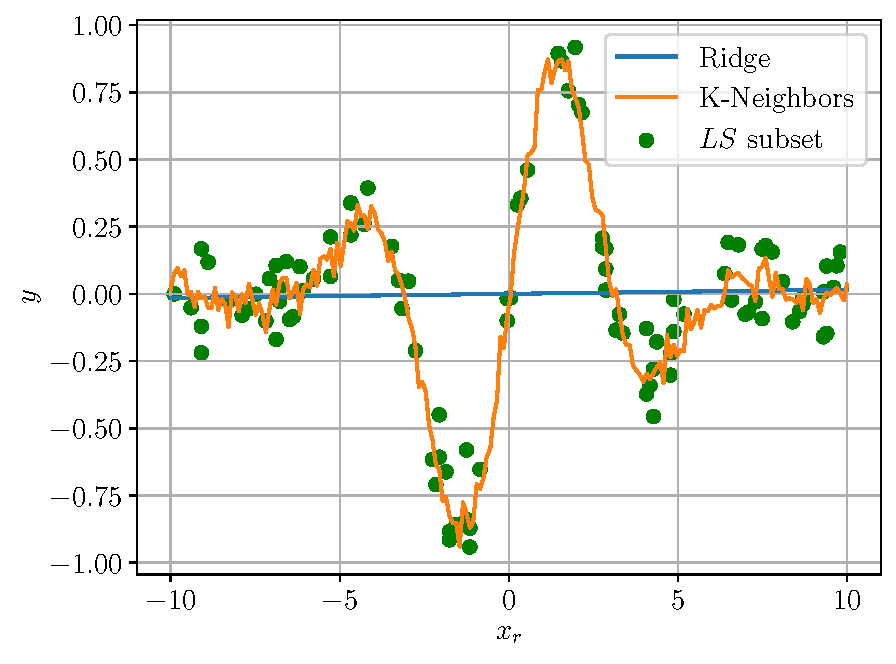
\includegraphics[width=0.66\textwidth]{resources/pdf/predictions.pdf}
            \vspace{-1em}
            \caption{Predictions of the Ridge ($\alpha = 1$) and K-Neighbors ($k = 5$) regressors trained with $LS$.}
            \label{fig:predictions}
        \end{figure}
        
        As one can see in Figure \ref{fig:predictions}, if the K-Neighbors method predicts quite well the overall shape of $f(x_r)$, it is not at all the case of the Ridge method which predicts $\hat{y}(x_r) \simeq 0$. This behavior was predictable since the more the linear model is tilted, the worse it predicts the most extreme (near $\pm 10$) points. Conversely, it doesn't predict that badly the center (near $0$) points with an almost null slope.

        Then, for both methods, a bias-variance decomposition (cf. Figures \ref{fig:ridge_d} and \ref{fig:k-nearest_d}) has been performed using the proposed protocol 3(a) for each $\bm{x}$ represented in $LS$.
        
        \begin{figure}[h]
            \centering
            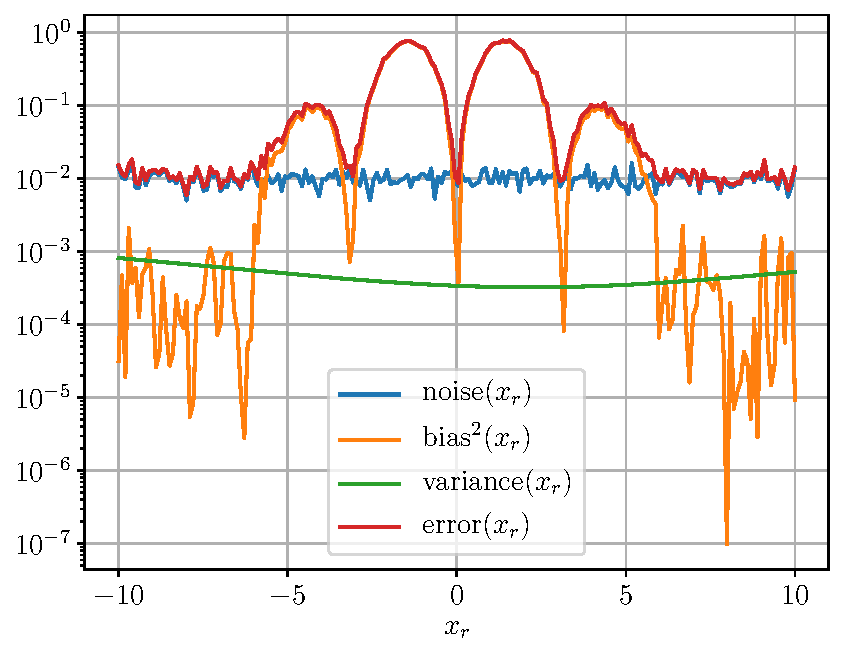
\includegraphics[width=0.66\textwidth]{resources/pdf/rrg.pdf}
            \vspace{-1em}
            \caption{Ridge regressor ($\alpha = 1$) trained with $LS$ bias-variance decomposition as a function of $x_r$.}
            \label{fig:ridge_d}
        \end{figure}
        
        For the linear regression method (cf. Figure \ref{fig:ridge_d}), as expected from the pace of its predictions, most of the error is concentrated around $x_r = 0$. Indeed, near the center, the (squared-)bias of the predictions is much greater due to the decreasing exponential and is, therefore, the main component of the global error.
         
        One can also observe in Figure \ref{fig:ridge_d} that the variance is quite low which means that the trained regressor doesn't vary much on the $p = 20$ learning sets of size $N / p$. Yet, the extremities varies more than the center which is very likely the result of a (slightly) varying slope.
        
        Finally, and this obviously hold for both methods, the estimated noise oscillates near the actual noise of the learning set, i.e. $0.1^2$.
        
        \begin{figure}[h]
            \centering
            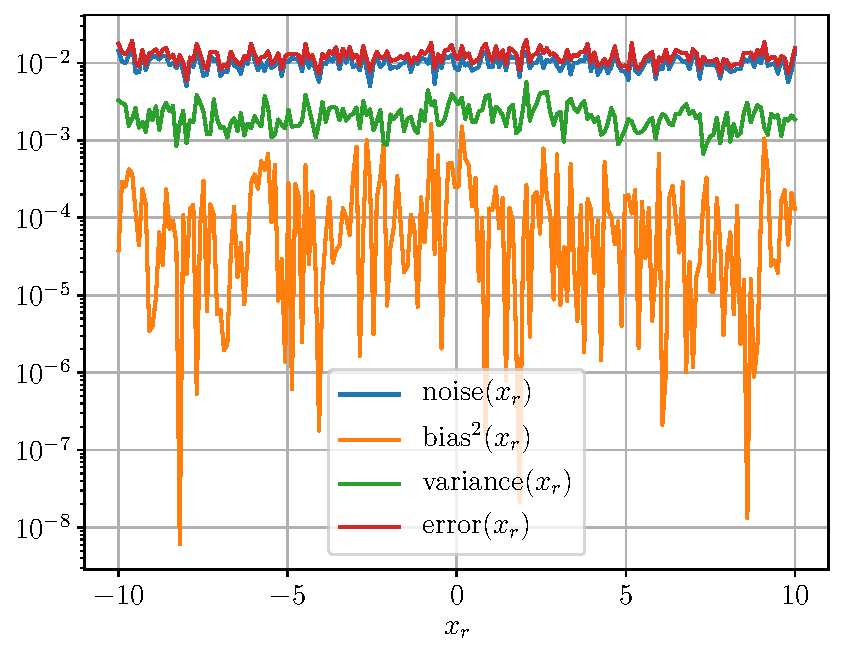
\includegraphics[width=0.66\textwidth]{resources/pdf/knr.pdf}
            \vspace{-1em}
            \caption{K-Neighbors ($k = 5$) trained with $LS$ bias-variance decomposition as a function of $x_r$.}
            \label{fig:k-nearest_d}
        \end{figure}
        
        For the non-linear regression method (cf. Figure \ref{fig:k-nearest_d}), neither the bias nor the variance seem significantly dependent on $x_r$. Moreover, the variance seems to oscillate around the value $\num{2e-3}$. This observation is supported by the theory\footnote{It is not the exact same case as in section \ref{sec:bias_variance_knn} since the input values $\bm{x}$ are not the same in each learning sample. However, because the size of each learning sample is far bigger (more than $k$ times) than the size of the discrete domain, it is very likely that the $k$ selected neighbors are the same; which is more or less the same assumption.} (cf. section \ref{sec:bias_variance_knn}) since the variance should equal $\frac{\text{noise}}{k} = \frac{0.1^2}{5}$. Concerning the bias, it is not surprising to obtain such low values since the predictions (cf. Figure \ref{fig:predictions}) are quite accurate.
        
        Because both bias and variance are lower than the noise, the later actually is the main component of the error. For this regression problem, the K-Neighbors ($k = 5$) regressor is preferable to the Ridge ($\alpha = 1$) one.
        
        \item To estimate the mean values of the noise, squared-bias, variance and expected error, the protocol 3(b) has been used. These values are dependent on the size of the learning sample $N$, the number of irrelevant variables $q$ and the complexity (or parameters) of the regressor ($\alpha$ or $k$). For both regression methods, the mean values have been computed as functions of $N$, $q$ and the complexity (one at a time, while the two others are constant).
        
        Starting by the noise (cf. Figure \ref{fig:mean_noise}), one can observe that it tends towards its actual value ($0.1^2$) when $N$ increases. However, when $q$ increases, the size of the domain explodes exponentially and quickly surpasses $N$. Therefore from $q = 2$, there isn't anymore twice the same input $\bm{x}$ in the learning sample and all estimated noises are undefined and so do the mean noise. For convenience this undefined mean noise is represented as $0$.
        
         \begin{figure}[h]
            \centering
            \begin{subfigure}{0.48\textwidth}
                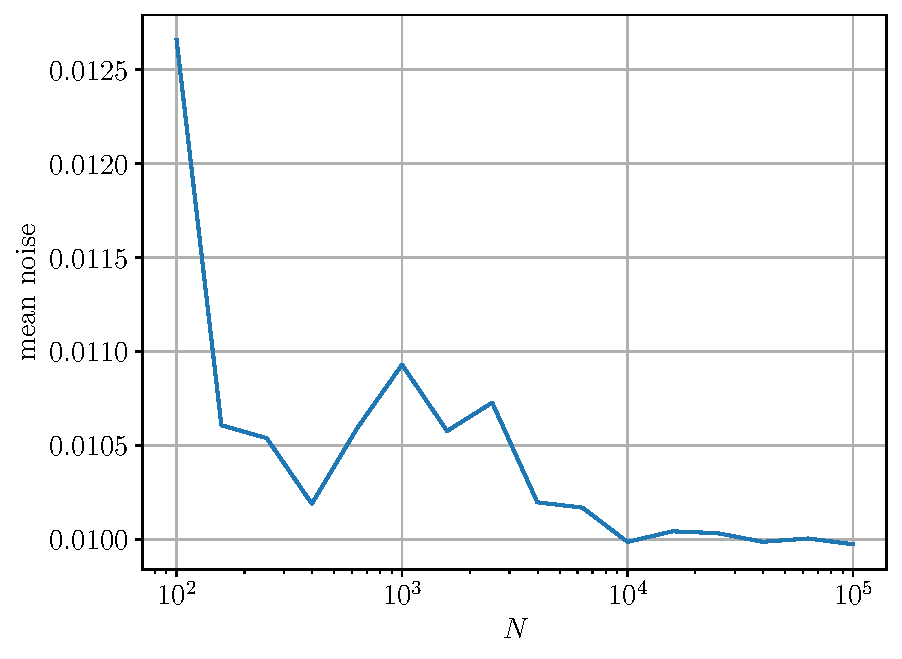
\includegraphics[width=\textwidth]{resources/pdf/mean_noise_n.pdf}
                \caption{$q = 0$}
            \end{subfigure}
            \begin{subfigure}{0.48\textwidth}
                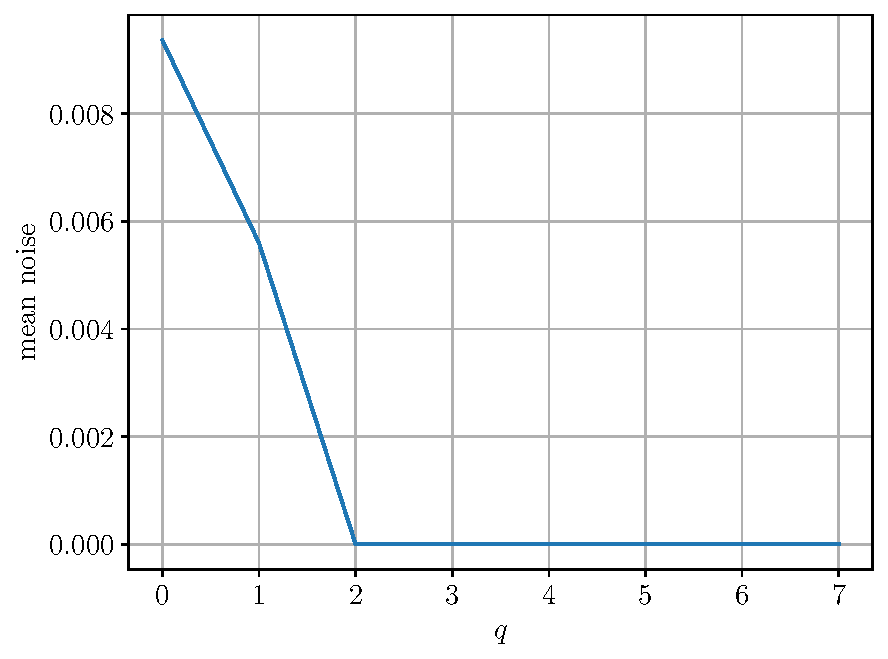
\includegraphics[width=\textwidth]{resources/pdf/mean_noise_q.pdf}
                \caption{$N = \num{e3}$}
            \end{subfigure}
            \caption{Mean noise as functions of $N$ and $q$.}
            \label{fig:mean_noise}
        \end{figure}
        
        It is not useful to plot the noise as a functions of the regressors complexity since it is independent of it, which is not the case of all other mean quantities (cf. \ref{fig:mean_error}).
        
        \begin{figure}[h]
            \centering
            \begin{subfigure}{0.48\textwidth}
                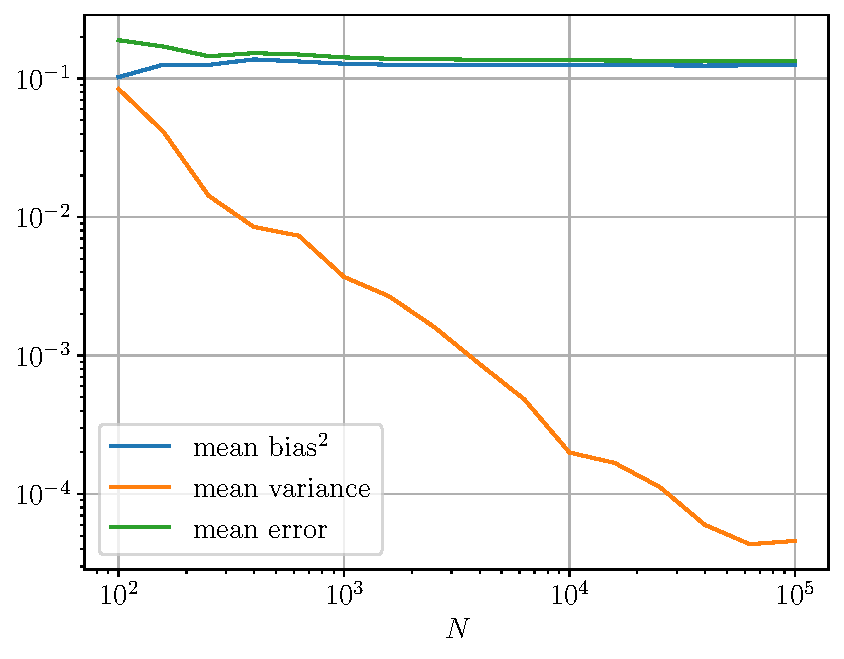
\includegraphics[width=\textwidth]{resources/pdf/rrg_mean_n.pdf}
                \caption{Ridge regressor, $q = 0$, $\alpha = 1$}
                \vspace{0.5em}
            \end{subfigure}
            \begin{subfigure}{0.48\textwidth}
                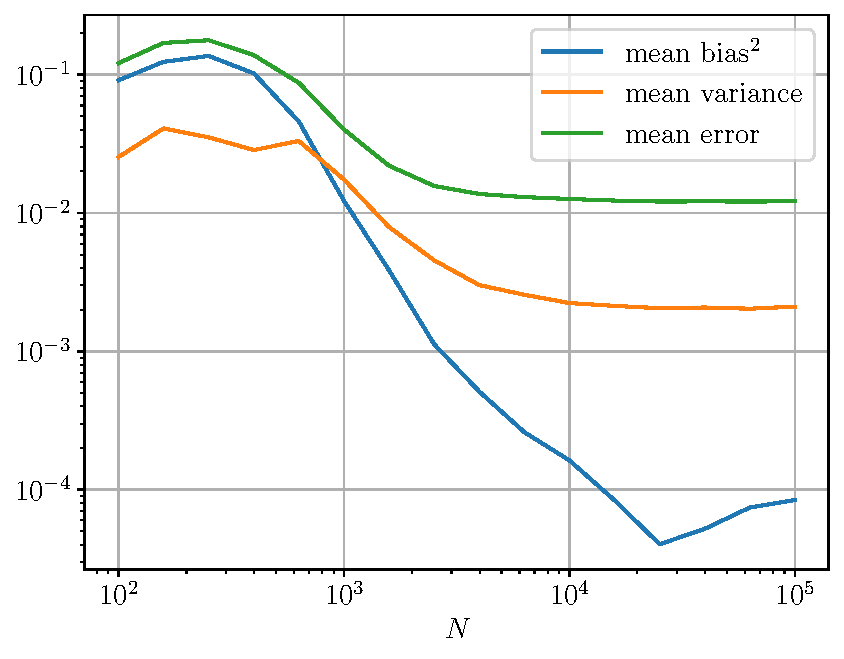
\includegraphics[width=\textwidth]{resources/pdf/knr_mean_n.pdf}
                \caption{K-Neighbors regressor, $q = 0$, $k = 5$}
                \vspace{0.5em}
            \end{subfigure}
            \begin{subfigure}{0.48\textwidth}
                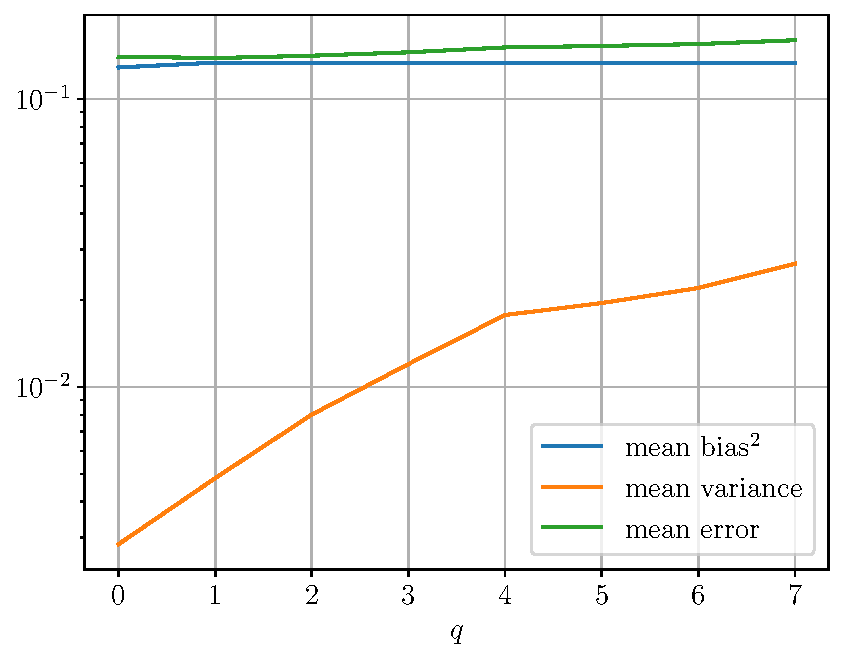
\includegraphics[width=\textwidth]{resources/pdf/rrg_mean_q.pdf}
                \caption{Ridge regressor, $N = \num{e3}$, $\alpha = 1$}
                \vspace{0.5em}
            \end{subfigure}
            \begin{subfigure}{0.48\textwidth}
                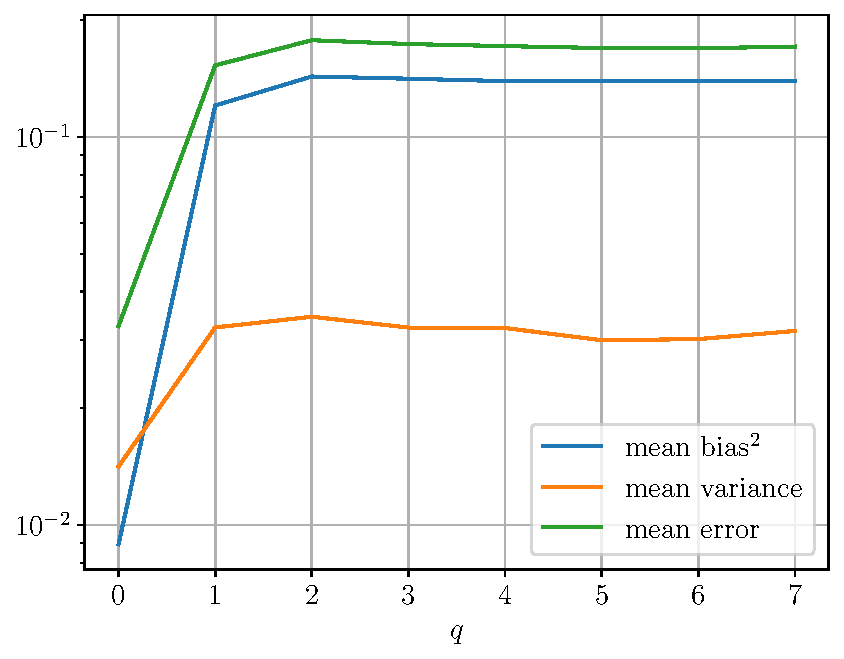
\includegraphics[width=\textwidth]{resources/pdf/knr_mean_q.pdf}
                \caption{K-Neighbors regressor, $N = \num{e3}$, $k = 5$}
                \vspace{0.5em}
            \end{subfigure}
            \begin{subfigure}{0.48\textwidth}
                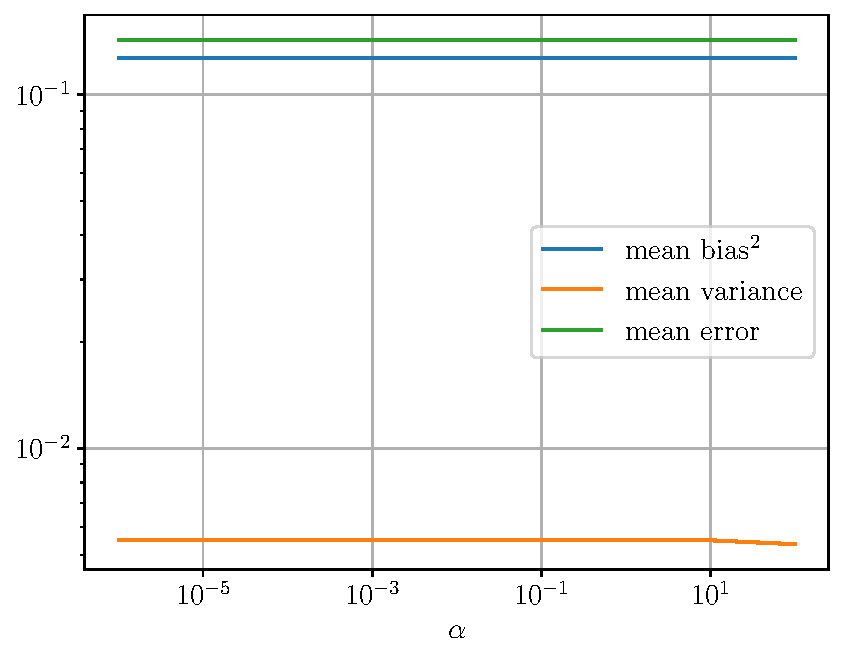
\includegraphics[width=\textwidth]{resources/pdf/rrg_mean_alpha.pdf}
                \caption{Ridge regressor, $N = \num{e3}$, $q = 0$}
            \end{subfigure}
            \begin{subfigure}{0.48\textwidth}
                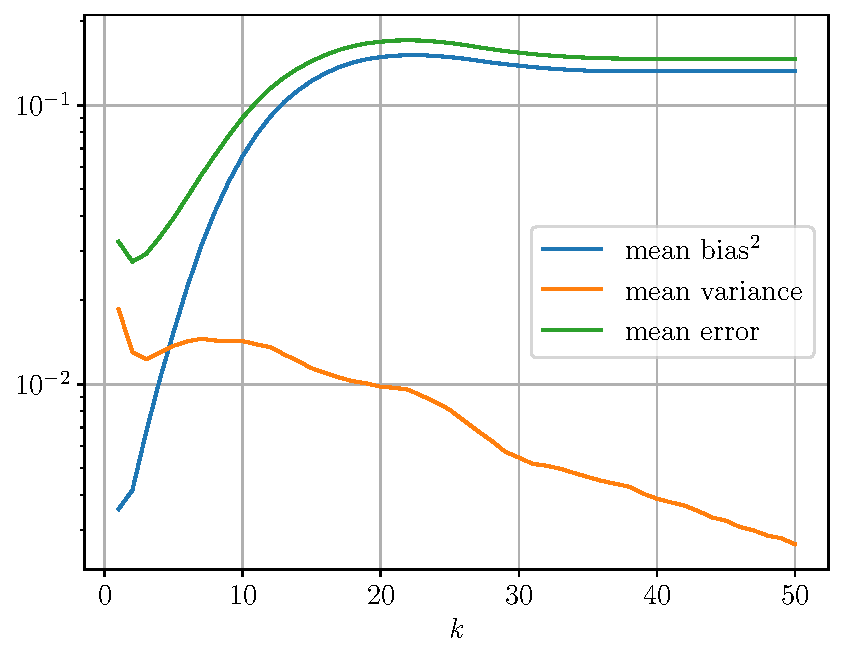
\includegraphics[width=\textwidth]{resources/pdf/knr_mean_k.pdf}
                \caption{K-Neighbors regressor, $N = \num{e3}$, $q = 0$}
            \end{subfigure}
            \caption{Mean squared-bias, variance and expected error as functions of $N$, $q$ and the complexity of the regressors.}
            \label{fig:mean_error}
        \end{figure}
        
        For the linear regression method, one can see that the three parameters ($N$, $q$ and $\alpha$) barely have an influence on the overall accuracy, especially $\alpha$ that has literally none. Conversely, as $N$ and $q$ increases, the mean variance of the model respectively drops and rises.
        
        Indeed, the coefficients of the Ridge regressor are heavily influenced by the spacial distribution of the learning set depending both on $N$ and $q$. Yet, the mean variance is too weak in comparison to the large mean squared-bias to be noticeable in the global mean error.
        
        For the non-linear regression method, it can be observed that all three parameters ($N$, $q$ and $k$) are determinant. As expected, when $N$ increases, the K-Neighbors regressor improves its accuracy (up to a certain lower limit) as a result of the more homogeneous coverage of the domain which directly influences the bias (nearer neighbors) and the variance (cf. footnote 4).
        
        When $q$ increases, the opposite effect occurs. Indeed, introducing irrelevant variables is misleading for the K-Neighbors algorithm since close neighbors in $q + 1$ dimensions might be far away in the first one (the relevant one). Therefore, if each input $\bm{x}$ isn't represented multiple times within the learning set, the $k$ nearest neighbors are selected more or less randomly regarding $x_r$ and $\hat{y}(\bm{x})$ tends toward the mean of $y$, that is $0$. Actually, one can draw a link between this behaviour and the predictions of the Ridge regressor. Indeed, the mean error and mean squared-bias of the K-Neighbors regressor for $q > 0$ and those of the Ridge regressor are very similar.
        
        The exact same behaviour can be observed as $k$ increases : $\hat{y}(\bm{x})$ tends toward the mean of $y$, i.e. $0$. However, if the variance remains more or less constant when $q$ grows, it is not the case with $k$ whose rise makes the variance decrease. 
    \end{enumerate}
\end{document}
